% Этот шаблон документа разработан в 2014 году
% Данилом Фёдоровых (danil@fedorovykh.ru) 
% для использования в курсе 
% <<Документы и презентации в \LaTeX>>, записанном НИУ ВШЭ
% для Coursera.org: http://coursera.org/course/latex .
% Исходная версия шаблона --- 
% https://www.writelatex.com/coursera/latex/5.1

\documentclass[t]{beamer}  % [t], [c], или [b] --- вертикальное выравнивание на слайдах (верх, центр, низ)
%\documentclass[handout]{beamer} % Раздаточный материал (на слайдах всё сразу)
%\documentclass[aspectratio=169]{beamer} % Соотношение сторон

%\usetheme{Berkeley} % Тема оформления
%\usetheme{Bergen}
%\usetheme{Szeged}

%\usecolortheme{beaver} % Цветовая схема
%\useinnertheme{circles}
%\useinnertheme{rectangles}

\usetheme{Berkeley}

%%% Работа с русским языком
\usepackage{cmap}					% поиск в PDF
\usepackage{mathtext} 				% русские буквы в формулах
\usepackage[T2A]{fontenc}			% кодировка
\usepackage[utf8]{inputenc}			% кодировка исходного текста
\usepackage[english,russian]{babel}	% локализация и переносы

%% Beamer по-русски
\newtheorem{rtheorem}{Теорема}
\newtheorem{rproof}{Доказательство}
\newtheorem{rexample}{Пример}

%%% Дополнительная работа с математикой
\usepackage{amsmath,amsfonts,amssymb,amsthm,mathtools} % AMS
\usepackage{icomma} % "Умная" запятая: $0,2$ --- число, $0, 2$ --- перечисление

%% Номера формул
%\mathtoolsset{showonlyrefs=true} % Показывать номера только у тех формул, на которые есть \eqref{} в тексте.
%\usepackage{leqno} % Нумерация формул слева

%% Свои команды
\DeclareMathOperator{\sgn}{\mathop{sgn}}

%% Перенос знаков в формулах (по Львовскому)
\newcommand*{\hm}[1]{#1\nobreak\discretionary{}
{\hbox{$\mathsurround=0pt #1$}}{}}

%%% Работа с картинками
\usepackage{graphicx}  % Для вставки рисунков
\graphicspath{{images/}{images2/}}  % папки с картинками
\setlength\fboxsep{3pt} % Отступ рамки \fbox{} от рисунка
\setlength\fboxrule{1pt} % Толщина линий рамки \fbox{}
\usepackage{wrapfig} % Обтекание рисунков текстом

%%% Работа с таблицами
\usepackage{array,tabularx,tabulary,booktabs} % Дополнительная работа с таблицами
\usepackage{longtable}  % Длинные таблицы
\usepackage{multirow} % Слияние строк в таблице

%%% Программирование
\usepackage{etoolbox} % логические операторы

%%% Другие пакеты
\usepackage{lastpage} % Узнать, сколько всего страниц в документе.
\usepackage{soul} % Модификаторы начертания
\usepackage{csquotes} % Еще инструменты для ссылок
%\usepackage[style=authoryear,maxcitenames=2,backend=biber,sorting=nty]{biblatex}
\usepackage{multicol} % Несколько колонок

%%% Картинки
\usepackage{tikz} % Работа с графикой
\usepackage{pgfplots}
\usepackage{pgfplotstable}

\title{Защита бакалаврской работы}
\subtitle{Исследование свойств оптических волокон с брэгговскими решётками для сенсорных применений}
\author[]{Барсегян Сергей Симонович\\[10mm]{\small научный руководитель: Дорофеенко Александр Викторович}}
\date{\today}
\institute[]{Московский физико-технический институт \\ Национальный исследовательский университет}


\AtBeginSection[]
{
	\begin{frame}<beamer>
		\frametitle{План}
		\tableofcontents
	\end{frame}
}

\begin{document}

\frame[plain]{\titlepage}	% Титульный слайд

\section{Введение}
\begin{frame}
	
	
\end{frame}	
\section{Мотивация}
\begin{frame}
	
\end{frame}	
\section{Эффект Кречмана}
\begin{frame}
	\begin{figure}[h]
		\centering
		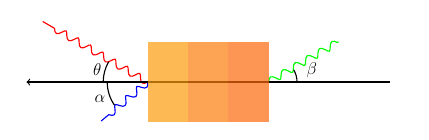
\includegraphics[width=1.1\linewidth]{screenshot006}
		\caption{}
		\label{fig:screenshot006}
	\end{figure}
\end{frame}

\begin{frame}
	
	\begin{figure}[h]
		\centering
		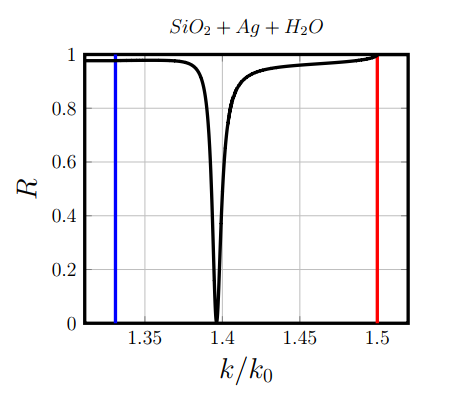
\includegraphics[width=0.7\linewidth]{screenshot004}
		\caption{}
		\label{fig:screenshot004}
	\end{figure}
	
\end{frame}	

\begin{frame}
	\begin{figure}[h]
		\centering
		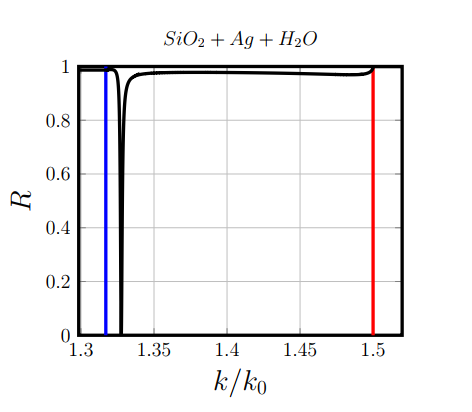
\includegraphics[width=0.7\linewidth]{screenshot005}
		\caption{}
		\label{fig:screenshot005}
	\end{figure}

\end{frame}

\section{Моды волновода}
\begin{frame}
	$$
	f_{m}(p)=\frac{J_{m}^{\prime}(p)}{p J_{m}(p)}, \quad g_{m}(q)=\frac{K_{m}^{\prime}(q)}{q K_{m}(q)} $$
	$$p=u a, q=v a $$
	$$p^{2}+q^{2}=a^{2}\left(k_{1}^{2}-k_{2}^{2}\right) $$
	$${\left[f_{m}(p)+g_{m}(q)\right]\left[\frac{\varepsilon_{1}}{\varepsilon_{2}} f_{m}(p)+g_{m}(q)\right]=\frac{m^{2} h^{2}}{k_{2}^{2}}\left(\frac{1}{p^{2}}+\frac{1}{q^{2}}\right)^{2}}
	$$
	
\end{frame}	
\section{Брэгговская решётка}
\begin{frame}
	
\end{frame}	
\section{Наклонная брэгговская решётка}
\begin{frame}
	
$$R=\tanh ^{2}(\kappa L)$$

$$\Delta n(x, y)=\Delta n \cos (4 \pi / \Lambda)(z \cos (\theta)+y \sin (\theta))$$
	
	
\end{frame}	

\begin{frame}
	
	$$\kappa=C \iint_{-\infty}^{\infty} \vec{E}_{\mathrm{core}}^{*} \cdot \vec{E}_{r} \Delta \mathrm{n}(\mathrm{x}, \mathrm{y}) \mathrm{d} \mathrm{xdy}$$
	
	\begin{figure}
		\centering
		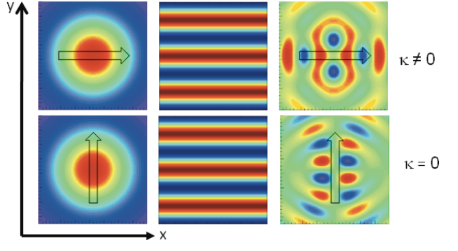
\includegraphics[width=0.7\linewidth]{screenshot001}
		\caption{}
		\label{fig:screenshot001}
	\end{figure}
	
	
\end{frame}	


\begin{frame}
	$$
	\Delta \lambda_{\mathrm{B}}=\left(2 \frac{N_{\mathrm{eff}}^{\text {core }} d \Lambda}{\cos (\theta)} \frac{d \Lambda}{d \varepsilon}+2 \frac{\Lambda}{\cos (\theta)} \frac{d N_{\text {eff }}^{\text {core }}}{d \varepsilon}\right) \Delta \varepsilon $$
	$$
	+\left(2 \frac{N_{\text {eff }}^{\text {core }}}{\cos (\theta)} \frac{d \Lambda}{d T}+2 \frac{\Lambda}{\cos (\theta)} \frac{d N_{\text {eff }}^{\text {core }}}{d T}\right) \Delta T $$
	$$
	\Delta \lambda^{\mathrm{r}}=\left(\frac{\left(N_{\text {eff }}^{\text {core }}+N_{\text {eff }}^{r}\right)}{\cos (\theta)} \frac{d \Lambda}{d \varepsilon}+\frac{\Lambda}{\cos (\theta)} \frac{d\left(N_{\text {eff }}^{\text {core }}+N_{\text {eff }}^{r}\right)}{d \varepsilon}\right)  \Delta \varepsilon $$
	$$
	+\left(\frac{\left(N_{\text {eff }}^{\text {core }}+N_{\text {eff }}^{r}\right)}{\cos (\theta)} \frac{d \Lambda}{d T}+\frac{\Lambda}{\cos (\theta)} \frac{d\left(N_{\text {eff }}^{\text {core }}+N_{\text {eff }}^{r}\right)}{d T}\right) \Delta T
	$$
	
	
	$$\Delta \lambda_{\mathrm{B}}-\Delta \lambda^{r}=\left(\frac{\left(N_{\mathrm{eff}}^{\mathrm{core}}-N_{\mathrm{eff}}^{r}\right)}{\cos (\theta)} \frac{d \Lambda}{d \varepsilon}\right) \Delta \varepsilon
	$$
\end{frame}	


\begin{frame}
\begin{figure}
		\centering
		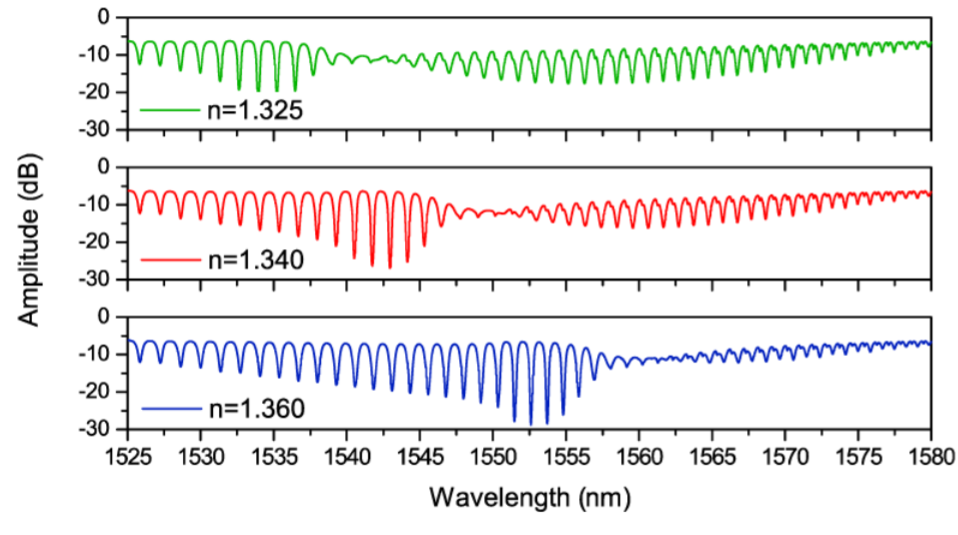
\includegraphics[width=0.7\linewidth]{screenshot002}
		\caption{}
		\label{fig:screenshot002}
\end{figure}
	

\end{frame}

\section{Дисперсия плазмона}
\begin{frame}
	
	\begin{figure}
		\centering
		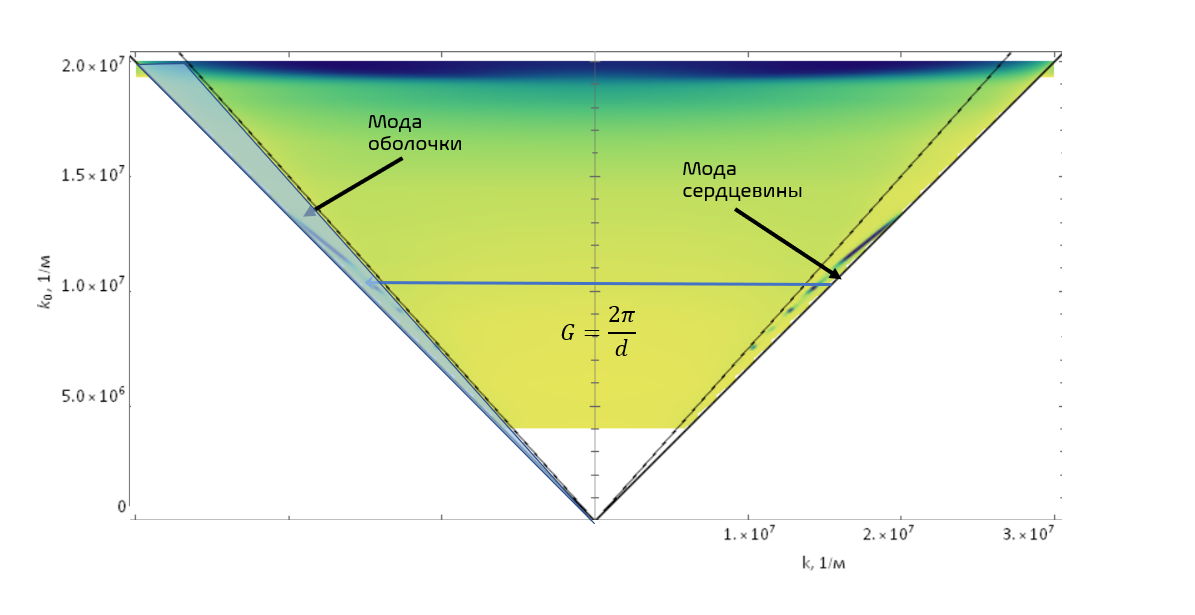
\includegraphics[width=1.0\linewidth]{screenshot003}
		\caption{Дисперсия плазмона}
		\label{fig:screenshot003}
	\end{figure}
	
	
\end{frame}	
\section{Заключение}
\begin{frame}
	
\end{frame}	



\end{document}